\documentclass[conference]{IEEEtran}
% CSD361 final report. Compile with pdfLaTeX (Overleaf default) + BibTeX:
%   pdflatex main && bibtex main && pdflatex main && pdflatex main
% Every number is traced to a committed file in report/NUMBERS.md.
\usepackage[T1]{fontenc}
\usepackage{cite}
\usepackage{amsmath,amssymb}
\usepackage{graphicx}
\usepackage{booktabs}
\usepackage{multirow}
\usepackage{xcolor}
\usepackage{algorithm}
\usepackage{algpseudocode}
\usepackage{tikz}
\usetikzlibrary{arrows.meta,positioning,fit}
\usepackage[hidelinks]{hyperref}

\newcommand{\ci}[3]{$#1$\,[$#2$,\,$#3$]}   % estimate [95% CI]
\newcommand{\dB}{\,dB}
\newcommand{\ID}{I_{\mathrm{D}}}
\newcommand{\IE}{I_{\mathrm{E}}}

\begin{document}

\title{Do Depth Priors and Gaussian Dropout Add Up in Sparse-View 3D Gaussian Splatting? A Pre-Registered Factorial and Bias--Variance Study}

\author{\IEEEauthorblockN{Aayush Trivedi (Roll No.\ 2410110012) \quad Disha Singh (Roll No.\ 2410110128)}
\IEEEauthorblockA{Department of Computer Science and Engineering, Shiv Nadar University, Delhi NCR, India\\
CSD361 -- Introduction to Machine Learning}}

\maketitle

\begin{abstract}
With only a few input views, 3D Gaussian Splatting (3DGS) overfits the training images and renders poor novel views. Two recent regularizers attack this from different sides: DNGaussian supervises the rendered depth with a monocular depth prior, and DropGaussian randomly drops Gaussians during training. We ask whether the two are complementary, redundant or interfering, and whether it matters if the dropout mask also reaches the depth supervision. We implement both in one code base and run a $2\times2$ factorial design (depth $\times$ dropout) plus a decoupled combination, with ablations of mask placement, dropout dose, depth weight, compensation and view count. The data are LLFF (8 scenes, 3 views), DTU (15 scans, 3 views) and Blender (8 objects, 8 views): 1,169 training runs with 3 seeds, analysed with decision rules fixed before the data existed. On LLFF, depth adds $+2.38$\dB{} PSNR and dropout $+0.48$\dB; adding dropout to DNGaussian gains $+0.50$ to $+0.60$\dB, and the two gains add up about additively. Across datasets the gain shrinks (pooled $+0.34$\dB{} [$+0.04$, $+0.64$] for the decoupled variant) and the interaction is never positive (pooled $-0.19$\dB{} [$-0.37$, $-0.01$]). Keeping the mask away from the depth passes has no measurable effect (pooled $+0.05$\dB{} [$-0.01$, $+0.12$]). A bias--variance split of the pixel mean squared error explains the pattern: in the sparsest settings depth mainly removes bias and dropout mainly removes run-to-run variance, yet variance remains 18--34\% of the combination's error. Most per-dataset interaction tests are inconclusive: with 8 scenes the smallest detectable interaction is 0.49\dB. The result is a careful, mostly null finding. Dropout is a cheap add-on to a depth prior in very sparse scenes, not a synergy.
\end{abstract}

\begin{IEEEkeywords}
Gaussian splatting, sparse-view novel view synthesis, regularization, dropout, bias--variance decomposition, factorial design
\end{IEEEkeywords}

%=====================================================================
\section{Introduction}
Novel view synthesis renders a scene from viewpoints that were never photographed. 3D Gaussian Splatting (3DGS)~\cite{kerbl2023gaussian} fits millions of 3D Gaussians to a set of posed photos and renders them in real time. With dozens of photos it works very well. With two or three, it overfits: many 3D scenes explain three photos equally well, and the optimizer picks one with floating, view-specific Gaussians and wrong geometry. Training images are reproduced almost perfectly while held-out views degrade. This is the classic gap between training and test error, and sparse-view methods are regularizers that close it.

Two recent regularizers take opposite routes. DNGaussian~\cite{li2024dngaussian} adds external knowledge: a monocular depth estimate~\cite{ranftl2021dpt} supervises the rendered depth. DropGaussian~\cite{park2025dropgaussian} adds structural noise: it removes a random subset of Gaussians at every training step, like dropout in neural networks~\cite{srivastava2014dropout}. Each helps on its own. A practitioner who wants both faces three questions that no published work answers: do their gains add up; do they overlap because they fix the same error; or do they interfere, for example because a random mask corrupts the depth supervision?

\textbf{Problem statement.} In sparse-view 3DGS, are DNGaussian's depth regularization and DropGaussian's Gaussian dropout complementary, redundant or interfering, and does it matter whether the dropout mask reaches the depth supervision?

\textbf{Objectives.} (O1)~Measure each regularizer's effect and their interaction. (O2)~Test where the mask should act. (O3)~Test whether the answer generalizes across datasets and view counts. (O4)~Explain the result with a bias--variance account of the test error. (O5)~Quantify the run-to-run noise and the statistical power, so that null results are interpretable.

\textbf{Approach.} Every variant is the same code with different flags. A $2\times2$ factorial design (depth on/off $\times$ dropout on/off) gives the main effects and an interaction contrast; a fifth variant keeps the mask away from the depth passes. All 1,169 runs came from tagged code, and the analysis rules were tagged before the data they govern existed.

\textbf{Contributions.}
\begin{itemize}
\item A controlled factorial measurement of the depth $\times$ dropout interaction on three datasets, with paired confidence intervals, equivalence margins and cross-dataset pooling (Sec.~\ref{sec:results}).
\item A placement study of where the mask acts, with a short analysis of why compensated dropout is biased under the rasterizer's opacity clamp. The prediction was tested and is not supported (Secs.~\ref{sec:method}, \ref{sec:ablation}).
\item A bias--variance error budget that explains where the two regularizers are complementary, and shows that the remaining error headroom is variance (Sec.~\ref{sec:budget}).
\item Noise-floor and power estimates for sparse-view evaluation, and a reproducible harness (tag-gated runner, checksummed data, CI-tested analysis) released with all run tables.
\end{itemize}

%=====================================================================
\section{Related Work}
\textbf{Radiance fields from sparse views.} NeRF~\cite{mildenhall2020nerf} represents a scene as a neural field; with few views it needs regularization, for example geometry and appearance priors on unobserved patches (RegNeRF~\cite{niemeyer2022regnerf}), a frequency schedule on the positional encoding (FreeNeRF~\cite{yang2023freenerf}) or a depth-ranking prior (SparseNeRF~\cite{wang2023sparsenerf}). 3DGS~\cite{kerbl2023gaussian} replaced the neural field with explicit Gaussians and rasterization. Its sparse-view variants add pseudo-views and depth (FSGS~\cite{zhu2024fsgs}) or co-regularize two Gaussian fields (CoR-GS~\cite{zhang2024corgs}).

\textbf{Base paper 1: DNGaussian.} DNGaussian~\cite{li2024dngaussian} regularizes sparse-view 3DGS with monocular depth from DPT~\cite{ranftl2021dpt}. Because monocular depth has unknown scale and shift, its loss compares depth patches after normalizing each by its own mean and spread, at a global and a local level. It renders depth in two extra passes per iteration, one that moves Gaussian centres (``hard'' depth, opacity fixed) and one that adjusts opacities (``soft'' depth), and uses a small neural field for colour.

\textbf{Base paper 2: DropGaussian.} DropGaussian~\cite{park2025dropgaussian} is prior-free. At each training step it drops every Gaussian with probability $r$ and scales the opacity of the survivors by $1/(1-r)$, as inverted dropout does~\cite{srivastava2014dropout}; $r$ grows linearly during training. The remaining Gaussians must explain the views on their own, which reduces overfitting.

\textbf{Dropout family and depth priors.} DropoutGS~\cite{xu2025dropoutgs} trains a randomly dropped sub-model against the full model and reports gains when plugged into other sparse-view pipelines. DropAnSH-GS~\cite{fang2026dropansh} argues that overlapping neighbours compensate for a dropped Gaussian and drops whole neighbourhoods instead. UGOD~\cite{guo2025ugod} learns uncertainty-guided opacity with soft dropout, and D$^2$GS~\cite{song2025d2gs} steers dropout by depth and density. On the depth side, StereoGS~\cite{yuan2026stereogs} uses stereo priors, and reliability-aware supervision~\cite{chu2026reliability} masks monocular depth where it is unreliable. Classical analyses read dropout as an adaptive regularizer that penalizes the variance of the output across masks~\cite{wager2013dropout}.

\textbf{Gap.} Several works stack dropout-style and depth regularization, or let depth steer the mask. None measures the \emph{interaction} of the two in a controlled design, separates where the mask acts, or reports the run-to-run noise that decides whether a small gain is real~\cite{bouthillier2021variance}. This project does all three, for the two base papers, on three datasets.

%=====================================================================
\section{Background and Problem Formulation}\label{sec:background}
\textbf{Rendering.} For one pixel's ray, let Gaussians $i=1,\dots,n$ be sorted front to back, each with per-pixel alpha $\alpha_i$ (opacity times its projected 2D falloff) and colour $c_i$. The pixel colour is
\begin{equation}
C=\sum_{i} c_i\,\alpha_i\,T_i,\qquad T_i=\prod_{j<i}(1-\alpha_j).
\label{eq:composite}
\end{equation}
Replacing $c_i$ by the view-space depth $z_i$ gives a depth map. The rasterizer clamps every alpha at $\alpha_{\max}=0.99$.

\textbf{Factorial contrasts.} Let A--D be the four cells of the $2\times2$ design (Table~\ref{tab:variants}) and E the decoupled combination. With each letter standing for a variant's mean PSNR on a scene, the main effects are $B-A$ (depth) and $C-A$ (dropout), and the interactions are
\begin{equation}
\ID=(D-C)-(B-A),\qquad \IE=(E-C)-(B-A).
\end{equation}
$I=0$ means the gains add up; $I<0$ means the combination gains less than the sum (overlap or conflict). $E-D$ measures the effect of keeping the mask off the depth passes.

\textbf{Verdicts.} A combination X $\in\{$D, E$\}$ is \emph{complementary} if it beats both B and C and its interaction is not negative; \emph{partly redundant} if its interaction is negative while it does not beat both; \emph{redundant} if it is equivalent to B with a negative interaction; \emph{interfering} if it is worse than B; otherwise \emph{inconclusive}. B (published DNGaussian) is the fixed reference.

\textbf{Bias and variance.} Training is stochastic (random initialization, random masks, and a nondeterministic GPU backward pass), so a variant's test error has two parts. With $n$ runs on fixed training views, renders $r_k$ and ground truth $y$, the expected single-run squared error of a pixel splits exactly into the squared error of the mean render (bias$^2$) and the spread between runs (variance):
\begin{equation}
\mathbb{E}_k(r_k-y)^2=(\bar r-y)^2+\mathrm{Var}_k(r_k).
\label{eq:bv}
\end{equation}
For a squared loss, training under random masks $m$ adds a penalty on the variance of the render across masks~\cite{wager2013dropout}:
\begin{equation}
\mathbb{E}_m\lVert y-\tilde R\rVert^2=\lVert y-\mathbb{E}_m\tilde R\rVert^2+\textstyle\sum_{\text{pixels}}\mathrm{Var}_m(\tilde R).
\label{eq:varpen}
\end{equation}
Depth, in contrast, adds information the views lack. We therefore expect depth to act mainly on bias and dropout mainly on variance; if they act on different components, their gains should add.

%=====================================================================
\section{Proposed Methodology}\label{sec:method}
Fig.~\ref{fig:workflow} shows the workflow, and Algorithm~\ref{alg:iter} one training iteration.

\begin{figure}[t]
\centering
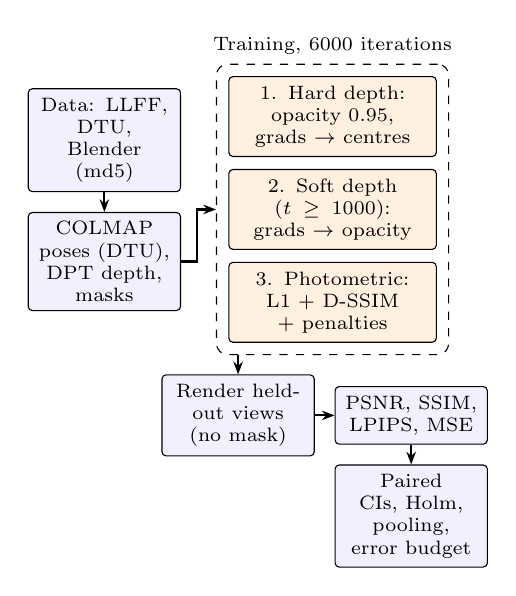
\begin{tikzpicture}[node distance=2.5mm and 2.5mm, font=\scriptsize,
  box/.style={draw, rounded corners=1.5pt, align=center, minimum height=7mm, text width=17mm, fill=blue!6},
  pass/.style={draw, rounded corners=1.5pt, align=center, minimum height=5mm, text width=24mm, fill=orange!12},
  ar/.style={-{Stealth[length=1.6mm]}, thick}]
\node[box] (data) {Data: LLFF, DTU, Blender (md5)};
\node[box, below=of data] (prep) {COLMAP poses (DTU), DPT depth, masks};
\node[pass, right=6mm of data, yshift=3mm] (hard) {1. Hard depth: opacity 0.95, grads $\to$ centres};
\node[pass, below=1.5mm of hard] (soft) {2. Soft depth ($t\ge1000$): grads $\to$ opacity};
\node[pass, below=1.5mm of soft] (photo) {3. Photometric: L1 + D-SSIM + penalties};
\node[draw, dashed, rounded corners, fit=(hard)(soft)(photo), inner sep=1.5mm, label={[font=\scriptsize]above:{Training, 6000 iterations}}] (train) {};
\node[box, below=4mm of photo, xshift=-12mm] (render) {Render held-out views (no mask)};
\node[box, right=of render] (eval) {PSNR, SSIM, LPIPS, MSE};
\node[box, below=of eval] (stats) {Paired CIs, Holm, pooling, error budget};
\draw[ar] (data) -- (prep);
\draw[ar] (prep.east) -- ++(2mm,0) |- (train.west);
\draw[ar] (train.south) ++(-12mm,0) -- (render.north);
\draw[ar] (render) -- (eval);
\draw[ar] (eval) -- (stats);
\end{tikzpicture}
\caption{Workflow. Each training iteration runs three rasterizations, each with its own backward pass. The dropout mask may reach any of them (Table~\ref{tab:variants}); rendering for evaluation never uses a mask.}
\label{fig:workflow}
\end{figure}

\textbf{Host: DNGaussian.} We use the authors' code. Every iteration runs three rasterizations, each with its own loss, backward pass and optimizer step: (1)~a \emph{hard-depth} pass with all opacities fixed at 0.95, whose depth loss moves only the centres; (2)~a \emph{soft-depth} pass from iteration 1000, with real opacities and detached geometry, whose depth loss changes only opacities; (3)~the \emph{photometric} pass, with L1 + $\lambda$\,D-SSIM and DNGaussian's shape, scale and opacity penalties. One weight $\lambda_d$ (\texttt{--depth\_scale}) multiplies both depth losses; $\lambda_d=0$ skips passes 1 and 2. On DTU a background-alpha term runs in every variant; on Blender the depth passes run every 10th iteration, as upstream.

\textbf{Dropout port.} We copy DropGaussian's two lines verbatim into the renderer: \texttt{comp = Dropout(p=r)(ones(N))} and \texttt{opacity = opacity * comp}, with schedule $r_t=\gamma\,t/10000$ and $\gamma=0.2$. 10000 is DropGaussian's iteration count; we keep it although we train for 6000 iterations, so the rate peaks at $r=0.12$. This keeps the published code unchanged; the dose block (Sec.~\ref{sec:ablation}) covers the published end rate $0.2$. One mask is drawn per iteration. With $\gamma=0$ no mask is created and the code reproduces DNGaussian exactly. The opacity penalty uses the opacity before dropout.

\begin{algorithm}[t]
\caption{One training iteration with mask routing}\label{alg:iter}
\small
\begin{algorithmic}[1]
\Require Gaussians $\mathcal G$, iteration $t$, dose $\gamma$, depth weight $\lambda_d$, routing $\rho\in\{$shared, clean, hard, soft$\}$
\State $r\gets\gamma t/10000$;\; $c\gets\mathbf 1$
\If{$\gamma>0$} draw $m_i\sim\mathrm{Bernoulli}(1-r)$;\; $c_i\gets m_i/(1-r)$ \EndIf
\If{$\lambda_d>0$}
  \State $c_h\gets c$ if $\rho\in\{$shared, hard$\}$ else $\mathbf 1$
  \State render depth with opacity $0.95\,c_h$; $\lambda_d\,\mathcal L_{\text{depth}}$; step centres
  \If{$t\ge1000$}
    \State $c_s\gets c$ if $\rho\in\{$shared, soft$\}$ else $\mathbf 1$
    \State render depth with opacity $\alpha\,c_s$; $\lambda_d\,\mathcal L_{\text{depth}}$; step opacities
  \EndIf
\EndIf
\State render image with opacity $\alpha\,c$; $\mathcal L_1+\lambda\,\mathcal L_{\text{D-SSIM}}+$ penalties; step all
\end{algorithmic}
\end{algorithm}

\textbf{Variants.} Table~\ref{tab:variants} lists them; all are flags of one code base. D lets one mask reach all three passes (the naive combination). E is decoupled: the depth passes always render all Gaussians. D\_hard and D\_soft let the mask reach only one depth pass, to localize any difference between D and E.

\begin{table}[t]
\caption{Variants (flags of one code base).}\label{tab:variants}
\centering\footnotesize\setlength{\tabcolsep}{3pt}
\begin{tabular}{@{}lccl@{}}
\toprule
ID & $\lambda_d$ & $\gamma$ & Mask reaches \\
\midrule
A & 0 & 0 & -- (3DGS host without depth) \\
B & 1 & 0 & -- (DNGaussian as published) \\
C & 0 & 0.2 & photometric (DropGaussian alone) \\
D & 1 & 0.2 & photometric, hard depth, soft depth \\
E & 1 & 0.2 & photometric only (decoupled) \\
D\_hard / D\_soft & 1 & 0.2 & photometric + one depth pass \\
\midrule
\multicolumn{4}{@{}l}{LLFF only: $\gamma\in\{0.1, 1/3\}$ (C, D, E); $\lambda_d\in\{0.5, 2\}$ (B, D);}\\
\multicolumn{4}{@{}l}{compensation \texttt{nc} / \texttt{clamp\_aware} (C, D); same-seed repeats.}\\
\bottomrule
\end{tabular}
\end{table}

\textbf{Why placement could matter: the alpha clamp.} With $\tilde\alpha_i=m_i\alpha_i/(1-r)$, $\mathbb E[\tilde\alpha_i]=\alpha_i$. Each term of \eqref{eq:composite} is a product of independent factors, so the expected masked render equals the clean one (\emph{Proposition~1}), as long as $\alpha_i/(1-r)\le\alpha_{\max}$. The rasterizer, however, computes $\min(\alpha_{\max},m_i\alpha_i/(1-r))$; when the clamp binds, $\mathbb E[\tilde\alpha_i]=(1-r)\alpha_{\max}<\alpha_i$. In the hard-depth pass every opacity is 0.95, so the clamp binds once $r>0.0404$, and the expected centre alpha falls to 0.931, 0.871 and 0.792 at $r=0.06$, 0.12 and 0.20. More light then passes to the Gaussians behind, so a masked hard pass is biased towards far depth. E's depth passes see no mask and no bias. This predicts $E>D$, with the deficit in D\_hard.

\textbf{Compensation modes} (LLFF). \texttt{uniform} is DropGaussian verbatim. \texttt{nc} uses the same draw, but survivors keep their opacity. \texttt{clamp\_aware} lowers each Gaussian's rate to $r_i=\min(r,1-\alpha_i/0.99)$, which makes compensation unbiased in every pass at the price of a smaller dose for opaque Gaussians.

\textbf{Error-budget estimator.} For each scene and variant we take the eval renders of the $n=3$ seeds. Per pixel and channel, with $\bar m$ the mean render and $s^2$ the sample variance across seeds,
\begin{equation}
\widehat{b^2}=(\bar m-y)^2-s^2/n,\qquad \widehat{\mathrm{var}}=s^2,
\end{equation}
so that the mean single-run MSE equals $\widehat{b^2}+\widehat{\mathrm{var}}$ exactly (the script asserts it). Terms are averaged over pixels, channels and views (DTU: inside the object mask). ``Variance'' is the spread between runs on fixed views; ``bias'' includes error no regularizer can remove, such as unseen regions. Averaging the 3 renders gives the ensemble error $(\bar m-y)^2$.

\textbf{Configuration.} All variants use DNGaussian's published settings per dataset for 6000 iterations from a random initial point cloud (Table~\ref{tab:hparams}).

\begin{table}[t]
\caption{Training settings (DNGaussian's published scripts).}\label{tab:hparams}
\centering\footnotesize\setlength{\tabcolsep}{2.5pt}
\begin{tabular}{@{}lccc@{}}
\toprule
 & LLFF & DTU & Blender \\
\midrule
Loss & L1 + 0.2 D-SSIM & L1 + 0.6 D-SSIM & L1 + 0.2 D-SSIM \\
Densify grad.\ threshold & 0.0013 & 0.001 & 0.0005 \\
Percent dense & 0.01 & 0.1 & 0.01 \\
Position lr & 0.016$\to$0.00016 & 0.0016$\to$1.6e-5 & 1.6e-4$\to$1.6e-6 \\
Scaling lr & 0.003 & 0.003 & 0.005 \\
Shape / opacity penalty & 0.002 / 0.001 & 0.005 / 0.001 & -- \\
Depth error tolerance & 0.00025 & 0.01 & 0.001 \\
\bottomrule
\end{tabular}
\end{table}

%=====================================================================
\section{Experimental Setup}\label{sec:setup}
\textbf{Datasets.} Table~\ref{tab:data} summarizes the three datasets. Each sample is a posed RGB image; the inputs are the training views with their camera poses and monocular depth maps; the target is the RGB image of each held-out view. LLFF~\cite{mildenhall2019llff} has 8 forward-facing real scenes (305 images, 20--62 per scene). DTU~\cite{jensen2014dtu} has object scans under controlled light; we use the 15 standard sparse-view scans (49 images each). The NeRF synthetic (Blender) set~\cite{mildenhall2020nerf} has 8 rendered objects with 100 training and 200 test images each. The data come from the official releases: LLFF and Blender from the NeRF authors, DTU ``Rectified'' from the DTU site, and the DTU evaluation masks from RegNeRF~\cite{niemeyer2022regnerf}.

\begin{table}[t]
\caption{Datasets and splits.}\label{tab:data}
\centering\footnotesize\setlength{\tabcolsep}{2.5pt}
\begin{tabular}{@{}lccc@{}}
\toprule
 & LLFF & DTU & Blender \\
\midrule
Scenes & 8 & 15 scans & 8 objects \\
Train views & 3 (also 2, 6, 9) & 3 (ids 25, 22, 28) & 8 \\
Test views & every 8th image & 25 & 25 (every 8th) \\
Resolution & $504\times378$ (1/8) & 1/4 & $400\times400$ (1/2) \\
Metrics & full image & object mask & full image \\
\bottomrule
\end{tabular}
\end{table}

\textbf{Preprocessing.} Camera poses come with LLFF and Blender. For DTU we ran COLMAP~\cite{schoenberger2016sfm} (4.2.1, CPU) through DNGaussian's converter. The DTU split selects views by index, so the pre-registered rule required all 49 images of a scan to register; all 15 scans did, four after the one allowed retry with a pinhole camera. Monocular depth for every training image came from DPT~\cite{ranftl2021dpt}, generated once per dataset and frozen in an archive that every machine checked by md5. A pre-registered go/no-go run of upstream DNGaussian on DTU scan 8 reached a masked PSNR of 19.11\dB, so DTU stayed in the study.

\textbf{Exploratory observation.} Training is not deterministic: the rasterizer's backward pass sums gradients with GPU atomic additions in a varying order. The same seed on the same GPU gave 17.75 and 17.29\dB{} on one scene in a short run, so every comparison averages over seeds and pairs by scene.

\textbf{Procedure.} Table~\ref{tab:blocks} lists the ten experiment blocks, 1,169 runs in all, with no failures and no reruns. Each block ran from a git tag with a clean tree (\texttt{v1.0-exp}, \texttt{v1.1-exp}, \texttt{v1.2-exp}); the runner refuses anything else and records the commit in every run. The analysis rules were tagged before the data they govern: \texttt{prereg-v1} before any LLFF metric, \texttt{prereg-v2} for compensation, and \texttt{prereg-v3} for DTU, Blender and the error budget, which was written after the LLFF results were seen and says so.

\begin{table}[t]
\caption{Experiment blocks (1,169 runs, 3 seeds unless noted).}\label{tab:blocks}
\centering\footnotesize\setlength{\tabcolsep}{2.5pt}
\begin{tabular}{@{}llrl@{}}
\toprule
Block & Variants / data & Runs & Tag \\
\midrule
T1 & A--E, LLFF 3v & 120 & v1.0 \\
P (pass) & D\_hard, D\_soft, LLFF 3v & 48 & v1.0 \\
G (dropout dose) & C, D, E at $\gamma$ 0.1, 1/3; seed 0 & 48 & v1.0 \\
N (noise) & B, D $\times$ 4 same-seed repeats, fern & 8 & v1.0 \\
V (views) & A--E, LLFF 2, 6, 9v & 360 & v1.0 \\
COMP & C, D $\times$ \texttt{nc}, \texttt{clamp\_aware} & 96 & v1.1 \\
DDOSE & B, D at $\lambda_d$ 0.5, 2 & 96 & v1.1 \\
NOISE2 & A--D $\times$ 4 repeats, 3 drawn scenes & 48 & v1.1 \\
DTU & A--E, 15 scans, 3v & 225 & v1.2 \\
Blender & A--E, 8 objects, 8v & 120 & v1.2 \\
\bottomrule
\end{tabular}
\end{table}

\textbf{Environment.} Python with PyTorch~\cite{paszke2019pytorch} 1.12.1 and DNGaussian's CUDA extensions, built from vendored sources. Every experiment trained on one NVIDIA RTX A4000 (16\,GB) in a lab PC. The \texttt{v1.0-exp} blocks ran one at a time; later blocks ran three at a time on the same GPU, which another user's process also occupied, so timing is reported only from T1. A 4\,GB laptop GPU and a Colab T4 served only for reproduction, smoke tests and data preparation.

\textbf{Metrics.} On held-out views: PSNR, SSIM~\cite{wang2004ssim} and LPIPS~\cite{zhang2018lpips} (VGG). DTU metrics are masked as in DNGaussian. For the error budget and scale checks, the pixel MSE and its root (RMSE) are regression metrics on the colour values in $[0,1]$. Geometry uses MVC@5\%, a multi-view depth consistency: the fraction of pixels whose rendered depth, reprojected into another held-out view, agrees with that view's depth within 5\%. It needs no ground truth.

\textbf{Statistics.} For each variant and scene we average over seeds; every comparison is a mean of per-scene differences with a 95\% $t$-interval over scenes. The three primary contrasts ($E-D$, $\ID$, $\IE$) are Holm-corrected~\cite{holm1979} per dataset. With margin $\delta=0.25$\dB, a contrast is ``$\approx 0$'' when its CI lies inside $\pm\delta$, and ``inconclusive'' when it crosses 0 and extends past $\pm\delta$; compensation contrasts add equivalence tests~\cite{lakens2017equivalence}. Datasets are pooled with a DerSimonian--Laird random-effects model~\cite{dersimonian1986}.

%=====================================================================
\section{Experimental Results and Discussion}\label{sec:results}

\begin{table*}[t]
\caption{Main results: mean over 3 seeds of the scene average ($\pm$ SD over seeds for PSNR). Best in bold. DTU metrics are masked.}\label{tab:main}
\centering\footnotesize\setlength{\tabcolsep}{4pt}
\begin{tabular}{@{}lccccccccc@{}}
\toprule
 & \multicolumn{3}{c}{LLFF, 3 views} & \multicolumn{3}{c}{DTU, 3 views} & \multicolumn{3}{c}{Blender, 8 views} \\
\cmidrule(lr){2-4}\cmidrule(lr){5-7}\cmidrule(l){8-10}
Variant & PSNR$\uparrow$ & SSIM$\uparrow$ & LPIPS$\downarrow$ & PSNR$\uparrow$ & SSIM$\uparrow$ & LPIPS$\downarrow$ & PSNR$\uparrow$ & SSIM$\uparrow$ & LPIPS$\downarrow$ \\
\midrule
A: none & 16.33 $\pm$ 0.23 & 0.460 & 0.394 & 14.04 $\pm$ 0.19 & 0.690 & 0.260 & 23.47 $\pm$ 0.04 & 0.879 & 0.098 \\
B: depth (DNGaussian) & 18.71 $\pm$ 0.04 & 0.592 & \textbf{0.302} & 18.37 $\pm$ 0.57 & 0.776 & 0.176 & 22.66 $\pm$ 0.03 & 0.868 & 0.112 \\
C: dropout & 16.80 $\pm$ 0.15 & 0.497 & 0.378 & 14.51 $\pm$ 0.48 & 0.726 & 0.243 & \textbf{23.83} $\pm$ 0.04 & \textbf{0.886} & \textbf{0.094} \\
D: both, shared mask & 19.21 $\pm$ 0.06 & 0.611 & 0.303 & 18.57 $\pm$ 0.26 & \textbf{0.810} & \textbf{0.160} & 22.77 $\pm$ 0.02 & 0.873 & 0.109 \\
E: both, decoupled & \textbf{19.31} $\pm$ 0.09 & \textbf{0.617} & 0.303 & \textbf{18.67} $\pm$ 0.17 & 0.807 & 0.163 & 22.82 $\pm$ 0.03 & 0.874 & 0.108 \\
\bottomrule
\end{tabular}
\end{table*}

\begin{table*}[t]
\caption{Paired PSNR contrasts (dB), mean over scenes with 95\% CI. Primaries ($E-D$, $\ID$, $\IE$) are Holm-corrected per dataset; ``$\approx$0'' = CI inside $\pm0.25$\,dB. Pooled: DerSimonian--Laird across the three datasets.}\label{tab:contrasts}
\centering\footnotesize\setlength{\tabcolsep}{4pt}
\begin{tabular}{@{}lcccc@{}}
\toprule
Contrast & LLFF (8 scenes) & DTU (15 scans) & Blender (8 objects) & Pooled \\
\midrule
$B-A$ (depth) & \ci{+2.38}{+1.80}{+2.96} & \ci{+4.34}{+3.25}{+5.42} & \ci{-0.80}{-1.78}{+0.18} & \ci{+1.96}{-0.56}{+4.48}, $\tau^2$ 4.81 \\
$C-A$ (dropout) & \ci{+0.48}{+0.18}{+0.77} & \ci{+0.48}{+0.01}{+0.95} & \ci{+0.37}{+0.19}{+0.55} & \ci{+0.40}{+0.28}{+0.53}, $\tau^2$ 0 \\
$D-B$ & \ci{+0.50}{+0.08}{+0.91} & \ci{+0.20}{-0.36}{+0.77} & \ci{+0.11}{-0.05}{+0.27} & \ci{+0.24}{-0.02}{+0.50} \\
$E-B$ & \ci{+0.60}{+0.30}{+0.91} & \ci{+0.30}{-0.09}{+0.68} & \ci{+0.15}{+0.02}{+0.28} & \ci{+0.34}{+0.04}{+0.64} \\
$E-D$ & \ci{+0.10}{-0.10}{+0.30} & \ci{+0.09}{-0.24}{+0.42} & \ci{+0.04}{-0.05}{+0.13} $\approx$0 & \ci{+0.05}{-0.01}{+0.12} $\approx$0 \\
$\ID$ & \ci{+0.02}{-0.34}{+0.38} & \ci{-0.28}{-0.85}{+0.30} & \ci{-0.26}{-0.37}{-0.15} & \ci{-0.19}{-0.37}{-0.01} \\
$\IE$ & \ci{+0.13}{-0.17}{+0.42} & \ci{-0.18}{-0.65}{+0.29} & \ci{-0.21}{-0.36}{-0.07} & \ci{-0.09}{-0.34}{+0.15} \\
\midrule
Verdict D / E & complementary / complementary & inconclusive / inconclusive & partly redundant / partly redundant & \\
\bottomrule
\end{tabular}
\end{table*}

\subsection{Main result on LLFF (O1)}
Table~\ref{tab:main} gives the main results and Table~\ref{tab:contrasts} the paired contrasts. On LLFF both regularizers help alone: depth by $+2.38$\dB{} and dropout by $+0.48$\dB. Adding dropout to DNGaussian helps: $D-B=+0.50$\dB{} and $E-B=+0.60$\dB, the latter in 8 of 8 scenes, and both combinations beat dropout alone by about 2.4\dB. Under the pre-registered rule both are therefore \emph{complementary}. The interactions are near zero and inconclusive in PSNR, so the gains add up about additively. In SSIM they are small but negative, with CIs that exclude 0 ($\ID=-0.018$ [$-0.032$, $-0.003$]): slightly sub-additive on that scale.

Our B (18.71\dB, 3 seeds, same pipeline and GPU as every other variant) is 0.41\dB{} below the published 19.12\dB~\cite{li2024dngaussian}; as a code check, a single-seed run of the upstream code over the 8 scenes on a Colab T4 gave a mean of 18.93\dB. DropGaussian's published 20.76\dB~\cite{park2025dropgaussian} uses its own 3DGS-based pipeline with a dense initialization and 10000 iterations, so it is not comparable to our C; we compare only our own controlled variants.

\subsection{Generalization across datasets (O3)}
Fig.~\ref{fig:forest} shows every contrast per dataset and pooled. Four patterns stand out. (i)~Dropout's own gain is consistent: $+0.37$ to $+0.48$\dB{} on every dataset, with no detectable heterogeneity ($\tau^2=0$). (ii)~Depth's gain is not: it is large on LLFF and DTU, but on Blender at 8 views it is inconclusive ($B-A=-0.80$ [$-1.78$, $+0.18$], 1 of 8 objects improves). There, dropout alone beats both combinations ($D-C=-1.06$ [$-2.07$, $-0.05$], $E-C=-1.02$ [$-2.01$, $-0.02$]; nominally significant, unadjusted). (iii)~Adding dropout to DNGaussian still helps pooled ($E-B=+0.34$\dB) and on Blender ($+0.15$\dB), by less than on LLFF. The pre-registered prediction that this gain is larger on DTU than on LLFF is not supported (one-sided Welch $p=0.82$). (iv)~The interaction is never positive: pooled $\ID=-0.19$\dB, with no significant heterogeneity (Cochran's $Q$, $p=0.21$), and on Blender both interactions are negative after Holm correction. On DTU all three primaries are inconclusive, because the 15 scans spread widely.

\begin{figure}[t]
\centering
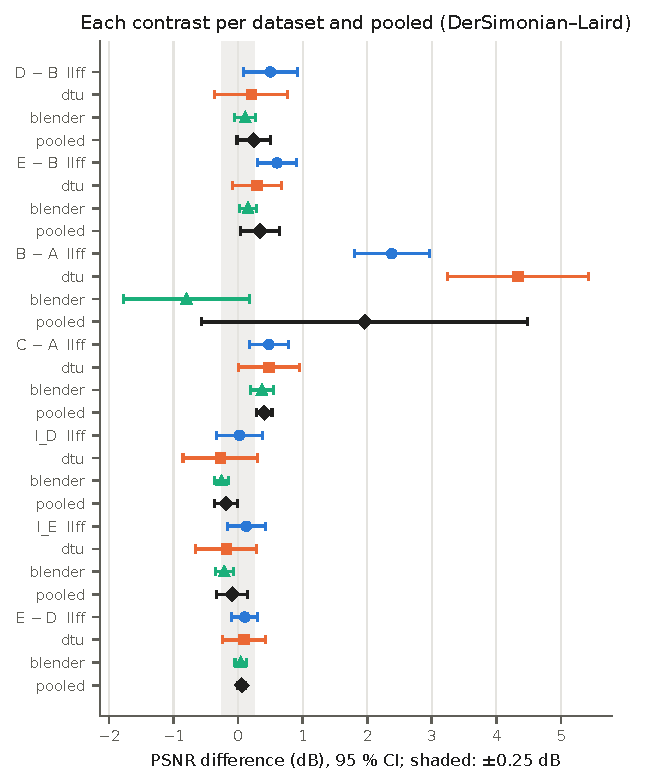
\includegraphics[width=0.86\columnwidth]{figures/fig_pooled.pdf}
\caption{PSNR contrasts per dataset and pooled (95\% CI; shaded: $\pm0.25$\,dB).}
\label{fig:forest}
\end{figure}

\subsection{Does the mask placement matter? (O2)}
$E-D$ is $\approx 0$ on Blender and pooled, and inconclusive on LLFF and DTU; every point estimate is between $+0.04$ and $+0.10$\dB. Pass localization finds no single pass responsible ($D_{\text{hard}}-E=-0.12$, $D_{\text{soft}}-E=-0.10$, both inconclusive; Table~\ref{tab:ablation}). On geometry the shared mask is, if anything, slightly better: MVC@5\% $E-D=-0.021$ [$-0.037$, $-0.005$], just past its margin of 0.02 (Holm $p=0.049$). At the published dose, letting the mask reach the depth passes neither helps nor measurably hurts.

\subsection{Why: the error budget (O4)}\label{sec:budget}
Fig.~\ref{fig:budget} and Table~\ref{tab:budget} split each variant's pixel MSE into bias$^2$ and run-to-run variance. Where the regularizers help, they act on different components. Depth's MSE reduction is mostly bias in the sparse settings (LLFF 2 and 3 views, DTU: bias share 0.51--0.96). Dropout's is mostly variance on LLFF up to 6 views and on Blender (variance share 0.74--0.84). This is the mechanism behind complementarity on LLFF.

The boundaries of the regime are as informative. At 6 and 9 views depth no longer reduces bias; at 9 views it increases bias, with a CI that excludes 0. On DTU, dropout's small PSNR gain is not a variance reduction (its MSE even rises slightly: PSNR and MSE disagree there). On Blender, depth raises the MSE, and its bias change is positive but not significant ($p=0.058$). Neither regularizer removes all the variance: in every setting the combination's MSE stays above DNGaussian's bias floor, variance is still 18--34\% of D's MSE, and averaging the renders of 3 seeds would gain $+0.57$ to $+1.10$\dB. The remaining headroom is variance, not bias.

The interaction is scale-dependent (Loftus~\cite{loftus1978}): on LLFF, $D-B$ and $E-D$ keep their sign under PSNR, MSE, RMSE and SSIM, but $\ID$ and $\IE$ do not. We therefore claim no more for the interaction than ``not positive''.

\begin{figure*}[t]
\centering
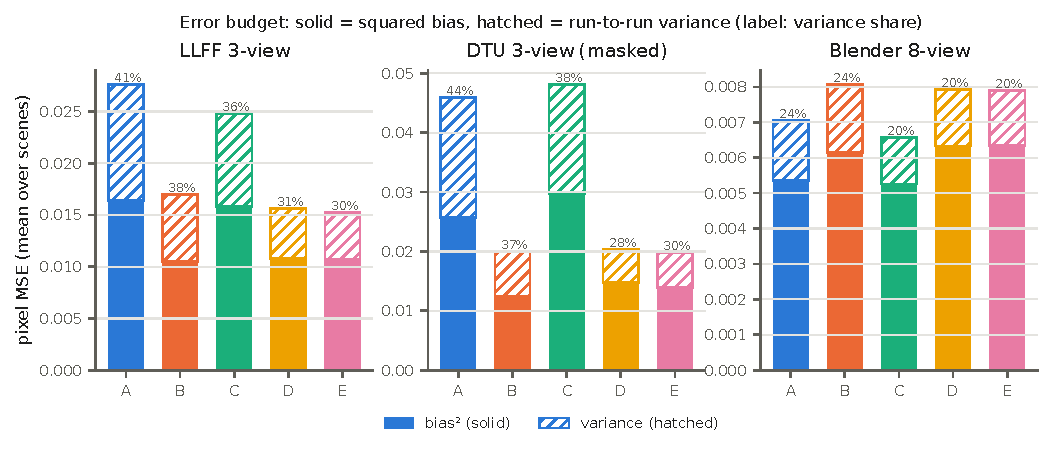
\includegraphics[width=0.78\textwidth]{figures/fig_budget.pdf}
\caption{Error budget: pixel MSE split into squared bias (solid) and run-to-run variance across 3 seeds (hatched); labels give the variance share.}
\label{fig:budget}
\end{figure*}

\begin{table}[t]
\caption{Error budget. Top: pixel MSE $\times10^3$ (variance share). Bottom: pre-registered tests (\checkmark holds, $\times$ fails) and D's ensemble gain.}\label{tab:budget}
\centering\footnotesize\setlength{\tabcolsep}{2.2pt}
\begin{tabular}{@{}lcccccc@{}}
\toprule
 & \multicolumn{4}{c}{LLFF} & DTU & Blender \\
\cmidrule(lr){2-5}
 & 2v & 3v & 6v & 9v & 3v & 8v \\
\midrule
A & 43.5 (31\%) & 27.6 (41\%) & 10.9 (42\%) & 7.37 (36\%) & 45.9 (44\%) & 7.05 (24\%) \\
B & 34.0 (39\%) & 17.0 (40\%) & 8.49 (28\%) & 7.13 (23\%) & 19.9 (37\%) & 8.08 (24\%) \\
C & 39.4 (26\%) & 24.8 (37\%) & 9.83 (38\%) & 7.05 (31\%) & 48.2 (39\%) & 6.58 (20\%) \\
D & 31.2 (33\%) & 15.6 (32\%) & 8.18 (22\%) & 7.07 (18\%) & 20.4 (28\%) & 7.93 (20\%) \\
E & 30.0 (34\%) & 15.2 (30\%) & 8.11 (22\%) & 7.09 (19\%) & 19.8 (28\%) & 7.91 (20\%) \\
\midrule
BV1 depth: bias share & 0.96\,\checkmark & 0.56\,\checkmark & 0.13\,$\times$ & $-2.90$\,$\times$ & 0.51\,\checkmark & 0.78\,$\times$ \\
BV2 dropout: var.\ share & 0.74\,\checkmark & 0.79\,\checkmark & 0.84\,\checkmark & 1.39\,$\times$ & $-0.76$\,$\times$ & 0.78\,\checkmark \\
BV3 MSE(D) $>$ bias$^2$(B) & yes & yes & yes & yes & yes & yes \\
D ensemble gain (dB) & 1.10 & 1.02 & 0.71 & 0.57 & 0.81 & 0.69 \\
\bottomrule
\end{tabular}
\end{table}

\subsection{Noise and power (O5)}
Repeating one seed varies as much as changing the seed: on fern the same-seed SD is 0.220\dB{} (B) and 0.216\dB{} (D), against between-seed SDs of 0.213 and 0.242\dB; on three more drawn scenes the same-seed/between-seed SD ratio of A--D lies between 1.00 and 1.67. Variants without depth are noisier: their run variance is 2.90 times that of the depth variants (SD about 1.7$\times$; one-sided $F$-test $p=2.5\times10^{-5}$). A single-run 8-scene mean is uncertain by $\pm0.26$\dB{} with depth and $\pm0.43$\dB{} without, the size of many published gains on LLFF 3-view. With 3 seeds, the smallest interaction detectable at 80\% power is 0.49\dB{} with 8 scenes, 0.33 with 15, 0.26 with 23 and 0.22 with all 31 pooled. This is why most per-dataset verdicts are ``inconclusive'' and only the pooled $\ID$ excludes 0.

\subsection{Discussion, limitations and challenges}
The two regularizers combine well only where each acts on a different error component: depth on bias, dropout on variance. That holds on LLFF at 2--3 views and fails as soon as depth stops removing bias (6--9 views, Blender) or dropout stops removing variance (DTU). The practical advice is modest: on very sparse inputs, add dropout to a depth-regularized model as is; the decoupled variant is not needed.

\emph{Limitations.} (i)~Power: interactions below about 0.5\dB{} are invisible per dataset, and ``inconclusive'' means ``not shown'', not ``absent''. (ii)~Nondeterminism and a shared GPU: the later blocks shared the GPU, so they give no efficiency numbers. (iii)~One dose: DropGaussian's schedule is kept verbatim (peak 0.12). (iv)~Blender uses one setting for all objects and the non-spherical-harmonics path, so B there is not tuned per object, and we compare DTU and Blender only with our own B. (v)~Post hoc elements: \texttt{prereg-v3} was written after the LLFF results were seen, and its variance-component check is circular by construction, so the power numbers are planning figures. Efficiency (T1, quiet GPU) is similar for B, D and E (141--145\,s per run, 39.6k--46.2k Gaussians).

%=====================================================================
\section{Ablation Analysis}\label{sec:ablation}

\begin{table}[t]
\caption{LLFF 3-view ablations: PSNR contrasts (dB) with 95\% CI.}\label{tab:ablation}
\centering\footnotesize\setlength{\tabcolsep}{3pt}
\begin{tabular}{@{}llc@{}}
\toprule
Ablation & Contrast & $\Delta$PSNR \\
\midrule
Pass (Holm, 2) & $D_{\text{hard}}-E$ & \ci{-0.12}{-0.32}{+0.08} \\
 & $D_{\text{soft}}-E$ & \ci{-0.10}{-0.27}{+0.07} \\
\midrule
Compensation & $C_{\text{nc}}-C$ & \ci{+0.14}{-0.10}{+0.38} \\
(Holm, 4) & $D_{\text{nc}}-D$ & \ci{-0.18}{-0.48}{+0.12} \\
 & $C_{\text{ca}}-C$ & \ci{-0.27}{-0.48}{-0.05} \\
 & $D_{\text{ca}}-D$ & \ci{-0.23}{-0.56}{+0.11} \\
\midrule
Depth weight & $\ID$ at $\lambda_d=0.5$ & \ci{+0.15}{-0.06}{+0.36} \\
 & $\ID$ at $\lambda_d=1$ & \ci{+0.02}{-0.34}{+0.38} \\
 & $\ID$ at $\lambda_d=2$ & \ci{-0.00}{-0.27}{+0.27} \\
\midrule
Dropout dose & $E-D$ at $\gamma=0.1 / 0.2 / 1/3$ & $-0.16$ / $+0.12$ / $+0.20$ \\
(seed 0) & $\ID$ at $\gamma=0.1 / 0.2 / 1/3$ & $+0.28$ / $+0.45$ / $-0.08$ \\
\bottomrule
\end{tabular}
\end{table}

\begin{table*}[t]
\caption{Number of training views (LLFF, 8 scenes, 3 seeds; 3 views = T1). Mean PSNR and paired contrasts with unadjusted 95\% CI.}\label{tab:views}
\centering\footnotesize\setlength{\tabcolsep}{4pt}
\begin{tabular}{@{}cccccccccc@{}}
\toprule
Views & A & B & C & D & E & $B-A$ & $D-B$ & $E-D$ & $\ID$ \\
\midrule
2 & 14.30 & 15.76 & 14.83 & 16.21 & 16.44 & \ci{+1.46}{+0.63}{+2.29} & \ci{+0.45}{+0.24}{+0.66} & \ci{+0.23}{-0.04}{+0.50} & \ci{-0.08}{-0.30}{+0.14} \\
3 & 16.33 & 18.71 & 16.80 & 19.21 & 19.31 & \ci{+2.38}{+1.80}{+2.96} & \ci{+0.50}{+0.08}{+0.91} & \ci{+0.10}{-0.10}{+0.30} & \ci{+0.02}{-0.34}{+0.38} \\
6 & 20.96 & 21.97 & 21.50 & 22.05 & 22.08 & \ci{+1.01}{+0.31}{+1.70} & \ci{+0.08}{-0.12}{+0.28} & \ci{+0.03}{-0.03}{+0.10} & \ci{-0.46}{-0.96}{+0.04} \\
9 & 22.85 & 22.64 & 22.91 & 22.60 & 22.55 & \ci{-0.20}{-0.73}{+0.32} & \ci{-0.04}{-0.18}{+0.10} & \ci{-0.05}{-0.19}{+0.09} & \ci{-0.10}{-0.34}{+0.14} \\
\bottomrule
\end{tabular}
\end{table*}

\textbf{Pass localization.} If the clamp bias mattered, masking only the hard-depth pass would carry D's deficit. Neither single-pass variant differs detectably from E (Table~\ref{tab:ablation}). A Monte-Carlo probe confirms the predicted far-depth shift under masking, larger at $r=0.20$ than at 0.12 in 8 of 8 scenes for D, but it is tiny: $+0.05\%$ of depth. The opacity-cap mechanism is not supported.

\textbf{Compensation.} Removing the $1/(1-r)$ rescaling (\texttt{nc}) or making it clamp-aware (\texttt{ca}) changes nothing significantly after Holm correction, and none of the four contrasts is shown equivalent to 0. Clamp-aware dropout tends to be worse ($C_{\text{ca}}-C=-0.27$, Holm $p=0.09$), the opposite of what the clamp explanation predicts.

\textbf{Depth weight.} Halving or doubling $\lambda_d$ leaves $\ID$ inconclusive at every weight; the pre-registered prediction that all three are $\approx 0$ does not hold, because the CIs are too wide to show equivalence.

\textbf{Dropout dose.} With one seed, $E-D$ rises with the dose ($-0.16$, $+0.12$, $+0.20$\dB{} at peak rates 0.06, 0.12 and 0.20), in 7 of 8 scenes. This is a trend, not a test; the other pre-registered conditions of the depth-corruption mechanism fail, so it is not supported.

\textbf{Number of views.} Table~\ref{tab:views} shows that the combination's benefit is a very-sparse effect: $D-B$ is $+0.45$ and $+0.50$\dB{} at 2 and 3 views and vanishes by 6. At 9 views depth is not shown to help ($B-A=-0.20$, inconclusive), like Blender at 8 views. The seed-0 interaction at 6 views ($-0.96$\dB) shrinks to $-0.46$\dB{} with three seeds and its CI includes 0, a reminder that single-seed effects of this size are unreliable.

\textbf{Test-time robustness.} Removing 20\% of the Gaussians at test time costs dropout-trained models about half as much PSNR as their dropout-free counterparts (C $-0.32$ vs A $-0.79$; D $-0.48$ vs B $-1.03$\dB): dropout makes the representation more redundant, as DropGaussian argues.

%=====================================================================
\section{Conclusion and Future Work}
We measured, under pre-registered rules and with 1,169 runs on three datasets, how DNGaussian's depth prior and DropGaussian's dropout combine in sparse-view 3DGS. Objective by objective: (O1)~met: each helps alone on LLFF and DTU, and on LLFF they add up about additively ($E-B=+0.60$\dB). (O2)~met, with a null result: where the mask acts makes no measurable difference, and the clamp and compensation explanations are not supported. (O3)~met: the benefit is confined to very sparse forward-facing scenes, and the pooled interaction is slightly negative. (O4)~partly met: depth removes bias and dropout removes variance where both help, but this split fails on DTU and at 6--9 views. (O5)~met: run noise of $\pm0.26$ to $\pm0.43$\dB{} and a detectable interaction of 0.49\dB{} at 8 scenes bound what any single dataset can show.

The main lesson is that the remaining error is variance, not bias. Future work: (i)~a per-scene detector that enables the depth loss only where it reduces bias; (ii)~combining depth with explicit variance reduction, such as seed ensembles or their distillation, to test whether the gap above DNGaussian's bias floor closes; (iii)~about 25 scenes per dataset (interpolated from the power analysis) to settle the sign of a 0.25\dB{} interaction.

\section*{Acknowledgment}
We thank the CSD361 course staff, the lab that provided the GPU, and the authors of DNGaussian and DropGaussian for releasing their code. Code, run tables and figures: \url{https://github.com/aayxsh23/dngs-dropout}.

\bibliographystyle{IEEEtran}
\bibliography{refs}

\end{document}
